\documentclass[a4paper,11pt]{article}
\pagestyle{headings}

\usepackage[utf8]{inputenc}
\usepackage[french]{babel}
\usepackage{graphicx}
\usepackage{float}
\usepackage[T1]{fontenc}
\graphicspath{{images/}}

\title{Optimisation parallèle de l'algorithme de Floyd-Warshall}
\author{Romain DULERY}
\date{\today}

\setlength{\oddsidemargin}{0.2cm}
\setlength{\evensidemargin}{-0.7cm}
\setlength{\parindent}{30pt}
\setlength{\textwidth}{15cm}
\setlength{\textheight}{24cm}
\setlength{\topmargin}{-.5in}
\setlength{\parskip}{1ex}

\begin{document}

\maketitle

\tableofcontents
\newpage

\section{Présentation générale du projet, objectifs et travail réalisé}

L'objectif du projet est d'optimiser l'algorithme de Floyd-Warshall à l'aide d'une implémentation parallèle, en OpenMP et OpenCL. L'accent sera mis sur l'optimisation spatiale de la mémoire, étant donné que l'algorithme est relativement simple et classique.\\\\
Les technologies utilisées sont C++11, OpenMP, Python3 pour les scripts, et Valgrind pour les analyses d'optimisation.\\\\
J'ai réalisé une plateforme de test de performance, pour générer automatiquement les données d'entrée, et les performances respectives des différents algorithmes.\\\\
Dans la partie suivante, sont présentées les méthodes de cette plateforme, le format de données utilisé, les scripts et un exemple d'exécution.\\\\

\section{Présentation de la plateforme de développement}

Elle se présente de la manière suivante :

\begin{figure}[H]
\begin{center}
  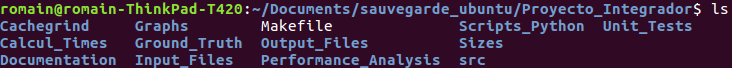
\includegraphics[scale=0.6]{arborescence.png}
  \caption{Arborescence utilisée}
\end{center}
\end{figure}

\subsection{Données d'entrée}

Celles-ci se trouvent dans le dossier Input\_Files.

\subsubsection{Format de données}

Le format choisi est le suivant :

La première ligne indique le nombre de sommets et d'arêtes.
Ensuite, chaque ligne représente une arête, avec le numéro du sommet initial, le numéro du sommet d'arrivée, et le poids associé à l'arête.

Les numéros de sommet commencent à 0.

\noindent Par exemple, ce graphe :

\begin{figure}[h]
\begin{center}
  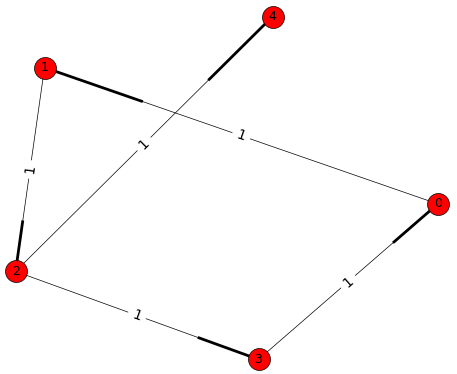
\includegraphics[scale=0.7]{input_exemple.png}
  \caption{Graphe d'exemple}
\end{center}
\end{figure}

\noindent Est représenté de la manière suivante :

\begin{figure}[h]
\begin{center}
  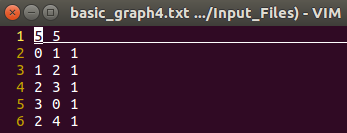
\includegraphics[scale=0.7]{input_graph4.png}
  \caption{Données d'entrée correspondantes}
\end{center}
\end{figure}

\subsubsection{Génération de données d'entrée}

Dans le dossier Scripts\_Python se trouvent les scripts \textbf{Input\_Files\_Generator.py} et \textbf{Special\_File\_Generator.py}, qui créent des données d'entrée.

Le premier génère 30 fichiers d'entrée. Les arguments sont le nom des fichiers générées, le nombre de sommets (aléatoire entre V/2 et V où V est l'argument), et le nombre d'arêtes en troisième argument, bien que celui-ci n'influe pas la complexité de l'algorithme, il sera quand même utile pour certains algorithmes. Le poids de chaque arête est aléatoire entre 1 et 100.

Le second script est le même que le premier, pour un seul fichier, avec un nombre exact de sommets et d'arêtes. Il sert à générer des graphes de référence.

\subsubsection{Données utilisées}

\noindent Dans tout le rapport, V représente le nombre de sommets, et E le nombre d'arêtes.

\noindent J'ai utilisé des graphes ordonnés en 7 catégories :

\begin{itemize}
  \item Basiques (basic\_graphX)\\\\
    Ils servent à tester le fonctionnement basique des algorithmes.
    Le graphe de la figure 2 est le basic\_graph4.\\

  \item Simples (simple\_graphX)\\\\
    V entre 5 et 20
    E entre 10 et 30\\

  \item Moyens (medium\_graphX)\\\\
    V entre 100 et 1000
    E entre 200 et 5000\\

  \item Complexes (complex\_graphX)\\\\
    V entre 2000 et 5000
    E entre 10000 et 50000\\

  \item Enormes (huge\_graphX)\\\\
    V entre 5000 et 10000
    E entre 50000 et 150000\\

  \item Références (reference\_graphX)\\\\
    Ce sont 6 graphes avec V = 400, 800, 1200, 1600, 2000 et 3200\\

Cela reste des graphes relativement petits pour pouvoir réaliser une comparaison pertinente des performances, notamment pour conjecturer le comportement lorsque V tend vers l'infini.

\end{itemize}

\subsection{Données de sortie}

Les données de sortie sont simplement la matrice de distances entre chaque sommet. Elles peuvent être sauvegardées dans des fichiers via une option du main, présentée dans la sous-partie suivante.

\subsection{Makefile et main}

Le main se génère via le \textbf{make}. Il peut être utilisé comme \textbf{make debug} ou \textbf{make sinopti}, pour générer le main en version débug, ou en version sans optimisation O3 du compilateur.

Le main demande un fichier d'entrée, et exécute chaque algorithme, en affichant les temps d'exécution de chaque algorithme sur la sortie standard.

\begin{figure}[H]
\begin{center}
  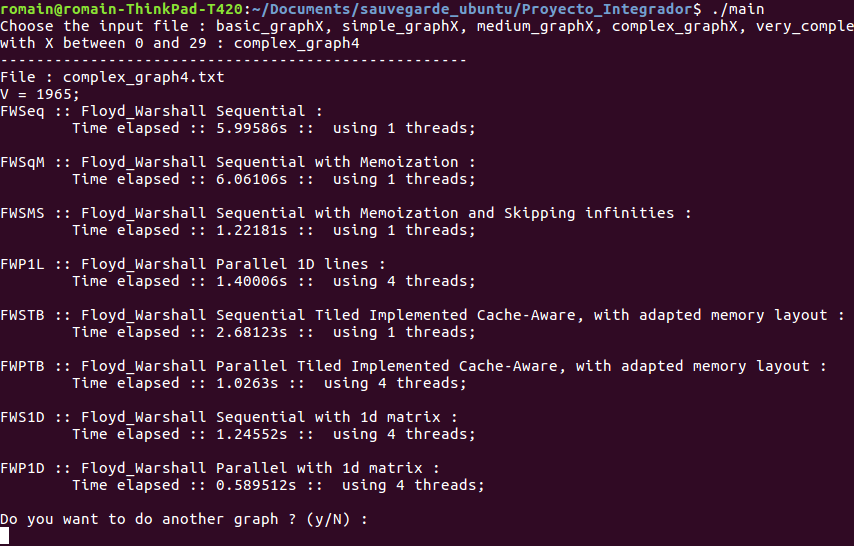
\includegraphics[scale=0.7]{main.png}
  \caption{Une exécution du main}
\end{center}
\end{figure}

\noindent Il possède également plusieurs options pour modifier le comportement, comme par exemple :

\begin{itemize}
    \item -a : pour choisir un seul algorithme
    \item -d : pour sauvegarder les données de sortie de chaque algorithme dans des fichiers, dans le dossier Output\_Files
    \item -t : pour sauvegarder les temps d'exécution pour chaque entrée dans des fichiers, dans le dossier Calcul\_Times
    \item -c : pour exécuter les algorithmes sur tous les fichiers d'entrée d'une catégorie (moyen, complexe..)
    \item -g : pour choisir le graphe d'entrée (sans que le main le demande, afin d'automatiser les résultats)
    \item -h : pour afficher l'aide
    \item -s : pour choisir le pas de certains algorithmes, présentés dans la partie suivante.
\end{itemize}

\section{Présentation de chaque algorithme}

Chaque algorithme est représenté par un code d'entrée et un code de sortie.

Le code d'entrée sert pour l'option -a du main, et le code de sortie sert pour l'option -t du main.

\subsection{Floyd-Warshall séquentiel}

\noindent Code d'entrée : FW\_SEQ \\
Code de sortie : FWSeq

\begin{figure}[H]
\begin{center}
  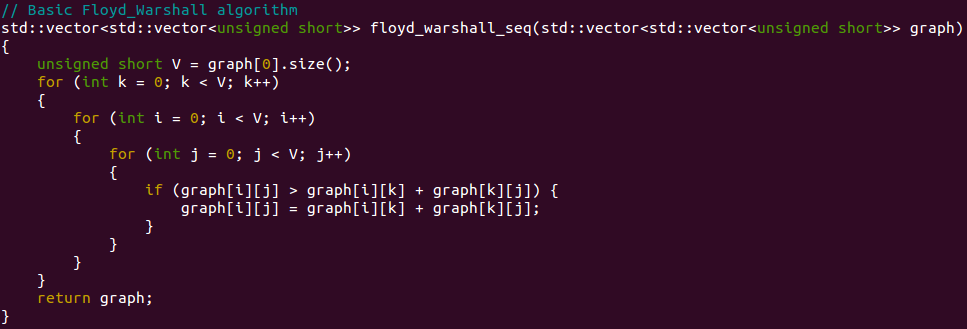
\includegraphics[scale=0.7]{FW_SEQ.png}
  \caption{Algorithme de Floyd-Warshall}
\end{center}
\end{figure}

C'est l'algorithme basique de Floyd-Warshall.

\subsection{Floyd-Warshall séquentiel avec mémoïzation}

\noindent Code d'entrée : FW\_SEQ\_MEM \\
Code de sortie : FWSqM

\begin{figure}[H]
\begin{center}
  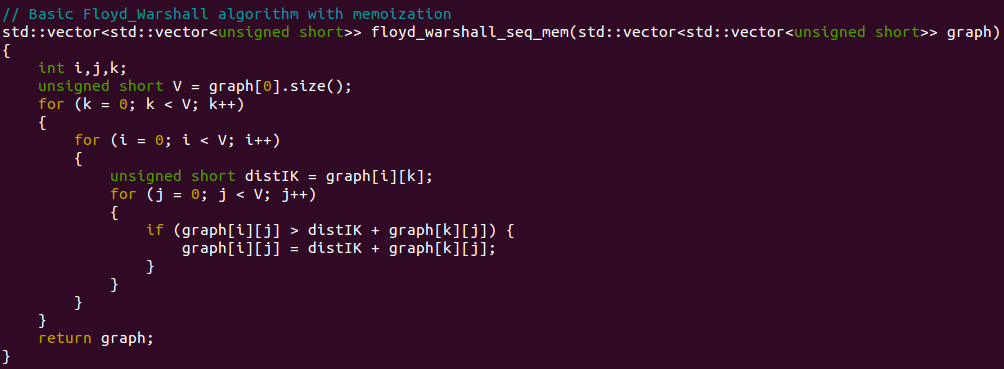
\includegraphics[scale=0.6]{FW_SEQ_MEM.png}
  \caption{Algorithme de Floyd-Warshall avec mémoïzation}
\end{center}
\end{figure}

C'est l'algorithme basique, avec mémorisation de la distance IK, qui est recalculée à chaque pour rien dans la dernière boucle sur j dans la version initiale.

Cela permet également de réduire le nombre de défauts de cache.

\subsection{Floyd-Warshall séquentiel avec mémoïzation et sauts d'infinis}

\noindent Code d'entrée : FW\_SEQ\_MEM\_SKIP \\
Code de sortie : FWSMS

\begin{figure}[H]
\begin{center}
  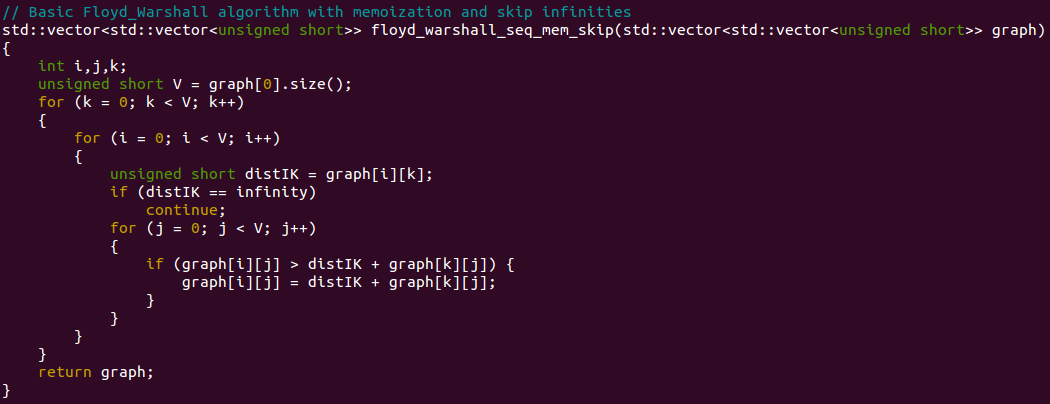
\includegraphics[scale=0.6]{FW_SEQ_MEM_SKIP.png}
  \caption{Algorithme de Floyd-Warshall avec mémoïzation et sauts d'infinis}
\end{center}
\end{figure}

C'est l'algorithme basique, avec mémoïzation de IK, et sauts d'infinis. Les sauts d'infinis font alors dépendre le temps de calcul du nombre d'arêtes, alors que normalement seul le nombre de sommets interviennent dans le calcul de la complexité.

Chaque algorithme qui suit utilisera les deux techniques de mémoïzation et sauts d'infinis.

\subsection{Floyd-Warshall parallélizé sur les lignes}

\noindent Code d'entrée : FW\_PAR1\_L \\
Code de sortie : FWP1L

\begin{figure}[H]
\begin{center}
  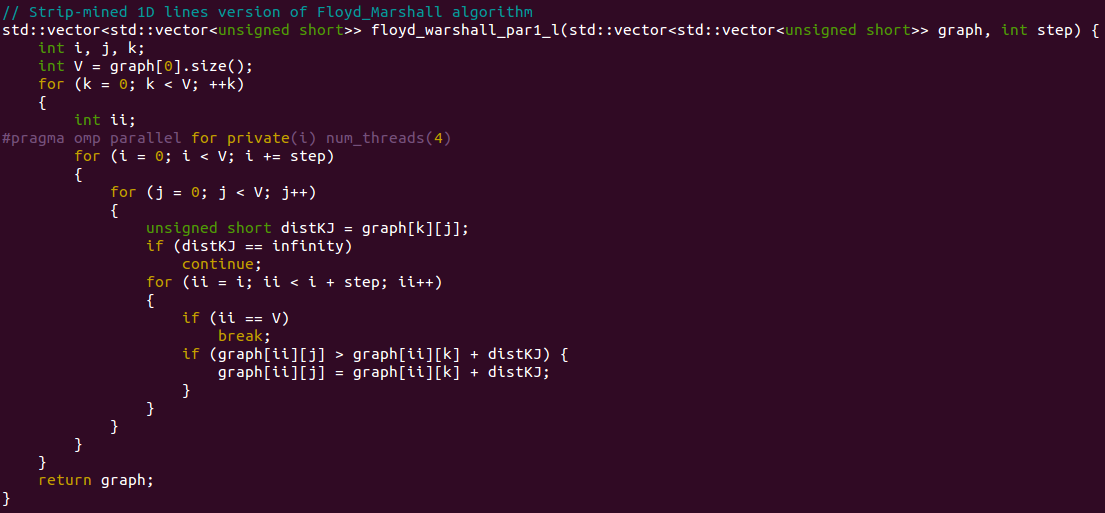
\includegraphics[scale=0.6]{FW_PAR1_L.png}
  \caption{Algorithme de Floyd-Warshall parallèle sur les lignes}
\end{center}
\end{figure}

La matrice est décomposée en bloc horizontaux, et chaque thread travaille sur un bloc.

\subsection{Floyd-Warshall parallélizé sur les colonnes}

\noindent Code d'entrée : FW\_PAR1\_C \\
Code de sortie : FWP1C

\begin{figure}[H]
\begin{center}
  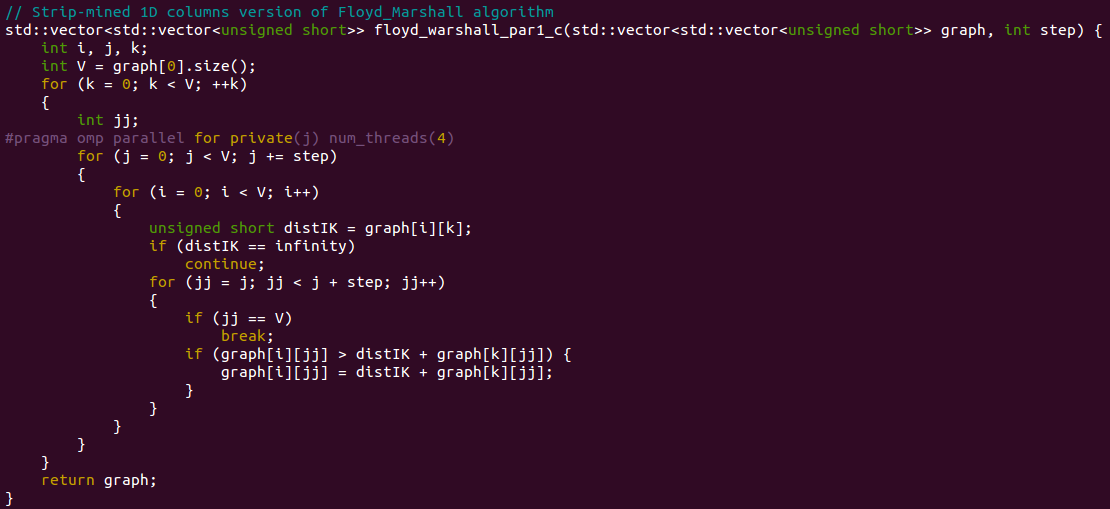
\includegraphics[scale=0.6]{FW_PAR1_C.png}
  \caption{Algorithme de Floyd-Warshall parallèle sur les colonnes}
\end{center}
\end{figure}

Idem que le précédent, sur les colonnes.

\subsection{Floyd-Warshall séquentiel, avec une matrice coupée en blocs carrés}

\noindent Code d'entrée : FW\_SEQ\_TILED \\
Code de sortie : FWSTI (Floyd-Warshall séquentiel "tiled-implemented")

\begin{figure}[H]
\begin{center}
  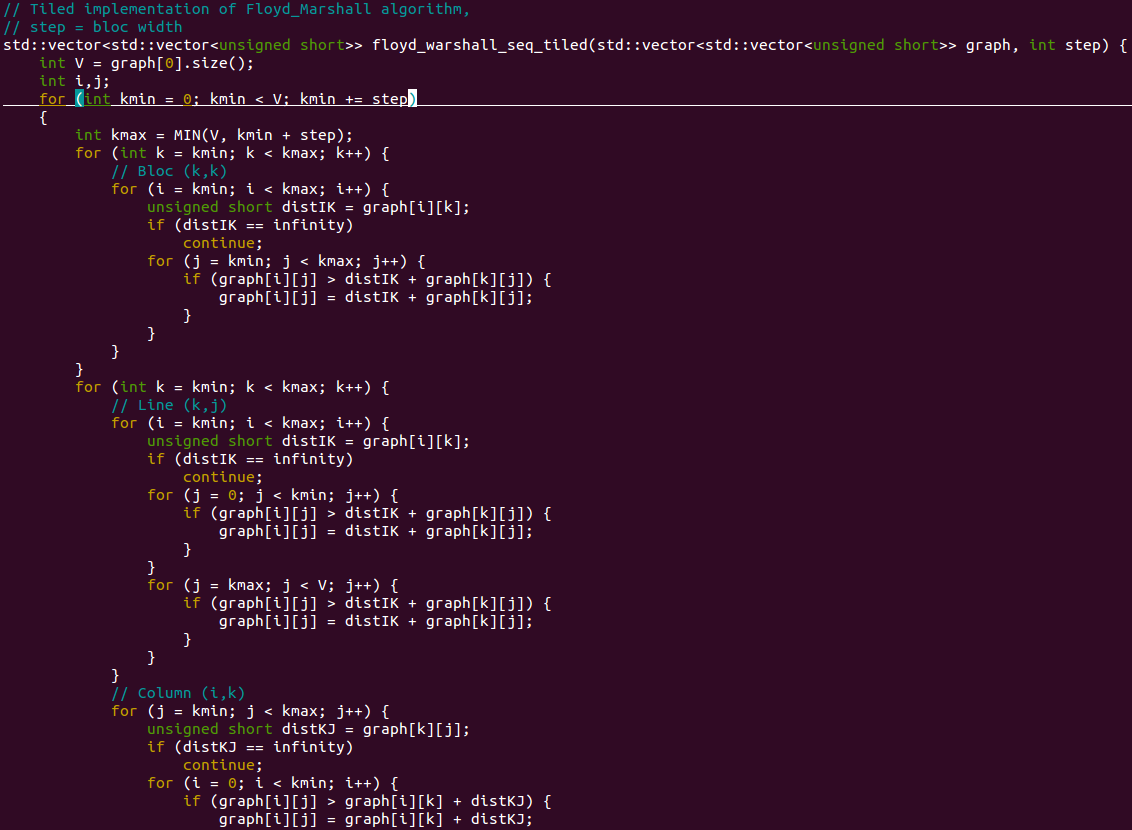
\includegraphics[scale=0.6]{FW_SEQ_TILED.png}
  \caption{Algorithme de Floyd-Warshall séquentiel en "tiled-implemented"}
\end{center}
\end{figure}

C'est un algorithme de transition vers l'algorithme suivant.

L'idée est de couper la matrice en blocs carrés, et de la traiter selon un ordre particulier :

\begin{minipage}{0.50\linewidth}
  \begin{enumerate}
    \item Le bloc (k, k)
    \item La ligne et la colonne du bloc, qui dépendent seulement du bloc (k,k)
    \item Ce qu'il reste
  \end{enumerate}
\end{minipage}\hfill
\begin{minipage}{0.4\linewidth}
  \begin{center}
    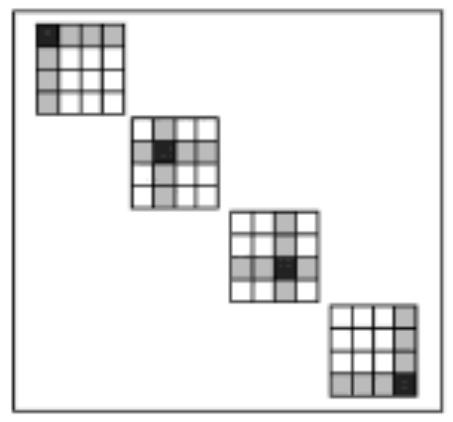
\includegraphics[scale=0.5]{FW_SEQ_TILED2.png}
  \end{center}
\end{minipage}
~\\\\\\
\indent Cet algorithme est fait pour qu'il soit cache-oblivious, de manière à ce qu'un bloc soit de la taille du cache. En effet, pour calculer chaque bloc, cela nécessite de charger seulement 1 bloc en étape 1, 2 bloc en étape 2, et 3 blocs en étape 3.

\subsection{Floyd-Warshall parallèle, avec una matrice coupée en bloc carrés}

\noindent Code d'entrée : FW\_PAR\_TILED \\
Code de sortie : FWPTI (Floyd-Warshall parallèle tiled-implemented)\\

C'est la version parallèle de l'algorithme précédent.

\subsection{Floyd-Warshall séquentiel, avec una matrice coupée en blocs carrés, avec une disposition adaptée de la mémoire}

\noindent Code d'entrée : FW\_SEQ\_TILED\_LAYOUT \\
Code de sortie : FWSTB (Floyd-Warshall séquentiel tiled-bloc implemented)

\begin{center}
  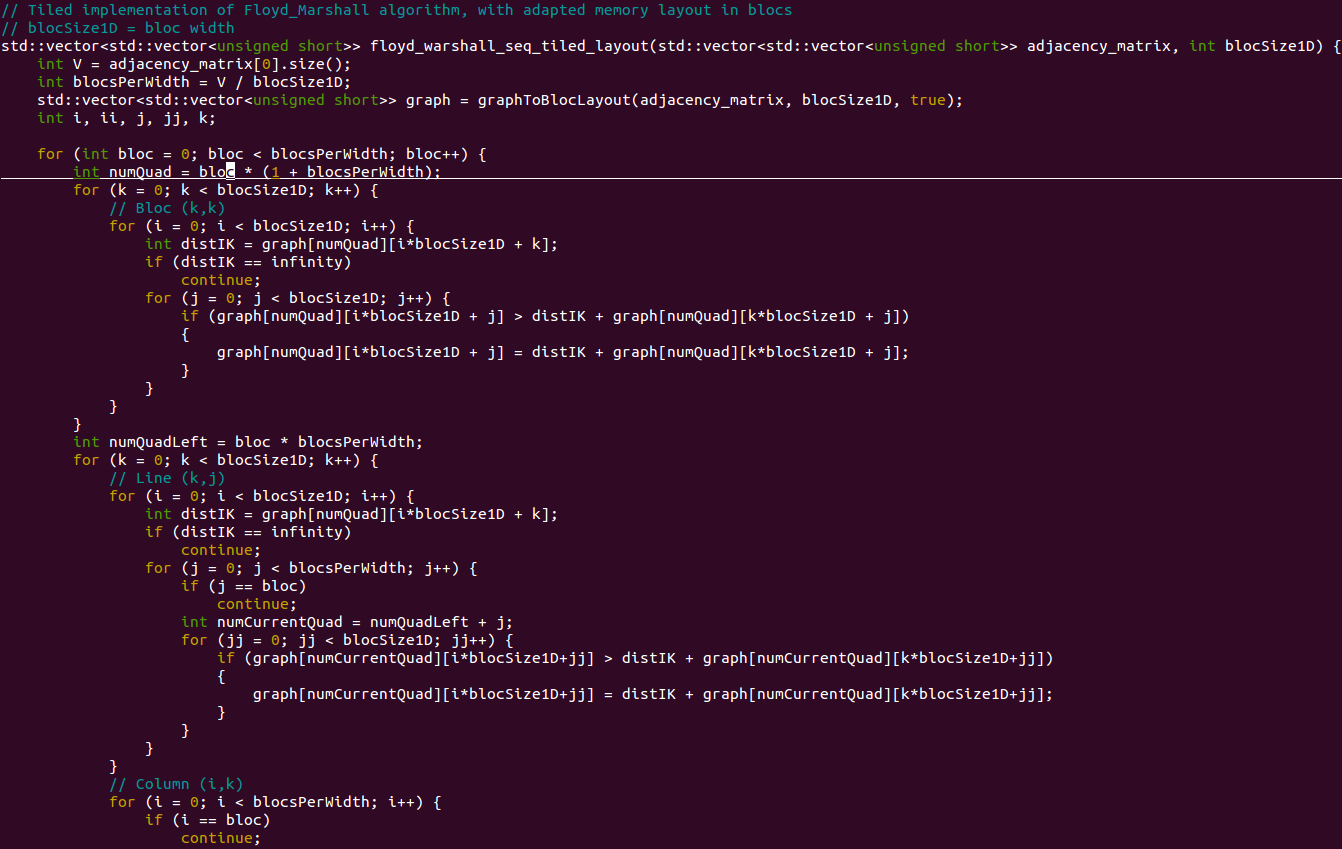
\includegraphics[scale=0.5]{FW_SEQ_TILED_LAYOUT.png}
\end{center}

C'est le même algorithme que précédemment, avec une disposition adaptée de la mémoire en blocs. C'est ce que la ligne 3 de l'algorithme fait.

L'idée est de réduire énormément le nombre de défauts de cache.

\subsection{Floyd-Warshall parallèle, avec una matrice coupée en blocs carrés, avec une disposition adaptée de la mémoire}

\noindent Code d'entrée : FW\_PAR\_TILED\_LAYOUT \\
Code de sortie : FWPTB (Floyd-Warshall parallel tiled-bloc implemented)\\

C'est la version parallèle de l'algorithme précédent. Cela devrait être le meilleur algorithme. Les algorithmes précédents ont été réalisés pour introduire cet algorithme.

\subsection{Floyd-Warshall séquentiel, avec une matrice en une dimension}

\noindent Code d'entrée : FW\_SEQ\_1D \\
Code de sortie : FWS1D

\begin{center}
  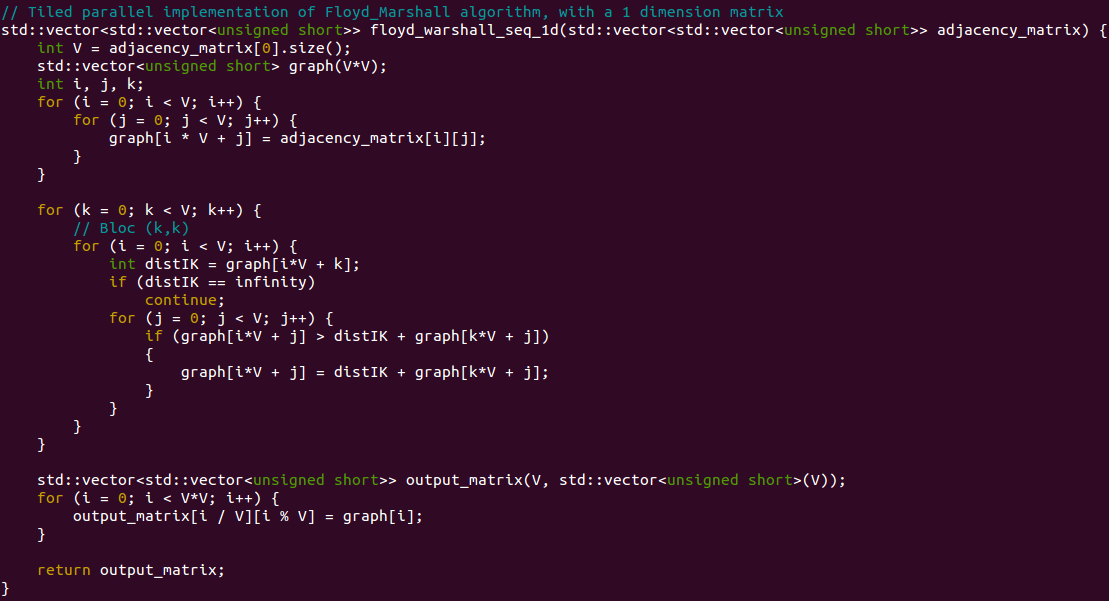
\includegraphics[scale=0.6]{FW_SEQ_1D.png}
\end{center}

C'est l'algorithme basique, avec une représentation 1D de la matrice.

Il peut se voir comme un cas particulier de l'algorithme précédent, quand il n'y a qu'un seul bloc.

\subsection{Floyd-Warshall parallèle, avec una matrice en une dimension}

\noindent Code d'entrée : FW\_PAR\_1D \\
Code de sortie : FWP1D

\begin{figure}[H]
\begin{center}
  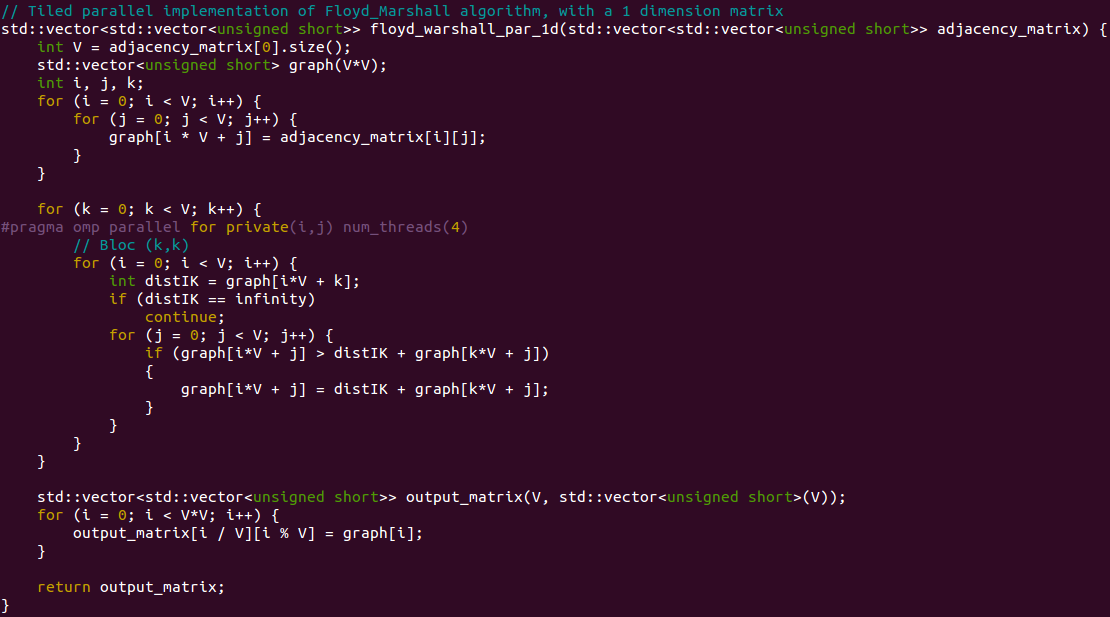
\includegraphics[scale=0.6]{FW_PAR_1D.png}
  \caption{Algorithme de Floyd-Warshall parallèle avec une matrice 1D}
\end{center}
\end{figure}

La version parallèle de l'algorithme précédent.

\section{Garantie de l'exactitude des sorties}
\subsection{Vérité Terrain}

J'ai commencé par vérifier les sorties de l'algorithme basique, qui peuvent être supposées correctes pour tout graphe si elles sont correctes sur les graphes basiques, étant donné que le code de l'algorithme est classique et se trouve facilement sur internet.

Le script Python \textbf{Verify\_Output.py} permet en effet de vérifier que les sorties pour les graphes basiques sont les mêmes que celles de la vérité terrain du dossier Ground\_Truth.

Pour vérifier les sorties basiques également, le script \textbf{Graph\_Generator.py} permet de générer des représentations visuelles de graphes, comme celui de la figure 2. Il a un intérêt que pour les graphes basiques.

\subsection{Script de comparaison des sorties}

Après l'utilisation de l'option -d du main (pour écrire les sorties des algorithmes dans des fichiers), il est possible de comparer les sorties de chaque algorithme.

\begin{minipage}{0.35\linewidth}
Le script à côté permet de faire des différences entre les fichiers de sortie du -d, pour vérifier que les algorithmes produisent bien la même sortie.\\

Si tous les algorithmes produisent la même sortie que l'algorithme basique, on suppose qu'ils sont exactes, même s'il peut y avoir des différences sur des cas limites, qui ne nous intéressent pas particulièrement dans ce projet.

\end{minipage}\hfill
\begin{minipage}{0.65\linewidth}
  \begin{center}
    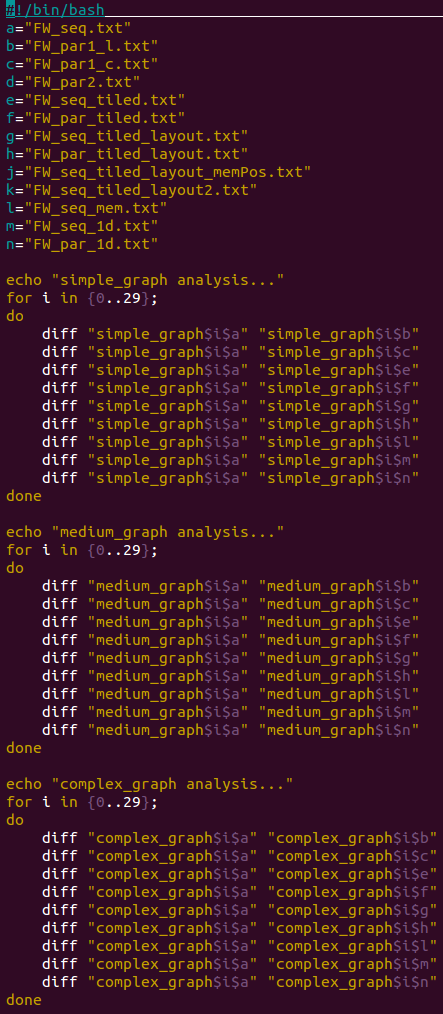
\includegraphics[scale=0.55]{diff_script.png}
  \end{center}
\end{minipage}

\section{Comparatif de performances}

Les comparatifs se font sur les graphes de taille au moins moyenne.

La configuration utilisée est la suivante :

\begin{itemize}
  \item Processeur : Intel(R) Core(TM) i5-3210M CPU @ 2.50GHz
  \item 4 threads
  \item Taille de cache : 3072 KB
  \item Compilateur : gcc 6.2
  \item Optimisation : O3
\end{itemize}

\subsection{Graphes moyens}

\begin{center}
  \begin{tabular}{p{2cm} | p{4.5cm} | p{2cm} | p{3cm} | p{3cm}}
    \centering \textbf{Algorithme} & \centering \textbf {Performances meilleures que l'algo basique} & \centering \textbf{Temps total} & \centering \textbf{Meilleur cas} & \centering \textbf{Pire cas} \tabularnewline
    \hline
    FWSeq & & 6.41 & & \\
    \hline
    \hline
    FWSqM & 29 & 6.24 & 118\% meilleur & 0\%, égual \\
    \hline
    FWSTB & 15 & 5.33 & 2308\% meilleur & 68\% pire \\
    \hline
    FWSTI & 23 & 2.95 & 4433\% meilleur & 64\% pire \\
    \hline
    FWP1C & 28 & 2.95 & 3640\% meilleur & 38\% pire \\
    \hline
    FWP1L & 30 & 2.80 & 4084\% meilleur & 16\% meilleur \\
    \hline
    FWS1D & 23 & 2.66 & 3913\% meilleur & 63\% pire \\
    \hline
    FWSMS & 30 & 2.48 & 17600\% meilleur & 17\% meilleur \\
    \hline
    FWPTB & 30 & 2.32 & 3379\% meilleur & 6\% meilleur \\
    \hline
    FWPTI & 29 & 1.39 & 5745\% meilleur & 60\% pire \\
    \hline
    FWP1D & 30 & 1.25 & 6946\% meilleur & 100\% meilleur \\
    \hline
  \end{tabular}
\end{center}

\subsection{Graphes complexes}

\begin{center}
  \begin{tabular}{p{2cm} | p{4.5cm} | p{2cm} | p{3cm} | p{3cm}}
    \centering \textbf{Algorithme} & \centering \textbf {Performances meilleures que l'algo basique} & \centering \textbf{Temps total} & \centering \textbf{Meilleur cas} & \centering \textbf{Pire cas} \tabularnewline
    \hline
    FWSeq & & 94.24 & & \\
    \hline
    \hline
    FWSqM & 25 & 93.97 & 2\% meilleur & 7\% pire \\
    \hline
    FWSTB & 16 & 74.94 & 4671\% meilleur & 47\% pire \\
    \hline
    FWP1C & 30 & 60.23 & 747\% meilleur & 1\% meilleur \\
    \hline
    FWP1L & 30 & 49.36 & 3891\% meilleur & 11\% meilleur \\
    \hline
    FWSTI & 30 & 44.19 & 6010\% meilleur & 12\% meilleur \\
    \hline
    FWSMS & 30 & 38.79 & 11861\% meilleur & 24\% meilleur \\
    \hline
    FWS1D & 30 & 38.69 & 6952\% meilleur & 24\% meilleur \\
    \hline
    FWPTB & 30 & 28.76 & 6318\% meilleur & 57\% meilleur \\
    \hline
    FWPTI & 30 & 20.88 & 7547\% meilleur & 100\% meilleur \\
    \hline
    FWP1D & 30 & 17.73 & 11506\% meilleur & 100\% meilleur \\
    \hline
  \end{tabular}
\end{center}

\subsection{Graphes très complexes}

\begin{center}
  \begin{tabular}{p{2cm} | p{4.5cm} | p{2cm} | p{3cm} | p{3cm}}
    \centering \textbf{Algorithme} & \centering \textbf {Performances meilleures que l'algo basique} & \centering \textbf{Temps total} & \centering \textbf{Meilleur cas} & \centering \textbf{Pire cas} \tabularnewline
    \hline
    FWSeq & & 1007 & & \\
    \hline
    \hline
    FWSTB & 2 & 1535 & 263\% meilleur & 54\% pire \\
    \hline
    FWP1C & 7 & 1243 & 33\% meilleur & 37\% pire \\
    \hline
    FWSqM & 20 & 1016 & 3\% meilleur & 8\% pire \\
    \hline
    FWP1L & 13 & 1006 & 107\% meilleur & 30\% pire \\
    \hline
    FWSTI & 30 & 729 & 232\% meilleur & 6\% meilleur \\
    \hline
    FWSMS & 30 & 706 & 215\% meilleur & 11\% meilleur \\
    \hline
    FWS1D & 30 & 694 & 263\% meilleur & 12\% meilleur \\
    \hline
    FWPTB & 29 & 589 & 641\% meilleur & 9\% meilleur \\
    \hline
    FWPTI & 30 & 365 & 585\% meilleur & 36\% meilleur \\
    \hline
    FWP1D & 30 & 335 & 647\% meilleur & 100\% meilleur \\
    \hline
  \end{tabular}
\end{center}

\subsection{Analyse}

\indent Cette partie est relativement uniquement à ma machine. Les résultats peuvent être très différents sur des machines plus puissantes.

L'algorithme parallèle avec la matrice en une dimension (et les deux optimisations basiques de mémoïzation et sauts d'infinis) est le meilleur.

C'est un cas particulier de l'algorithme en blocs, qui devrait théoriquement être meilleur. Par ailleurs l'algorithme FWPTI, qui est un FWPTB sans changer la représentation en mémoire de la matrice, fournit de meilleurs résultats. C'est un résultat étranger étant donné que l'algorithme est conçu pour utiliser une représentation spatiale différente des données, de plus, avec gprof il est possible de voir que les fonctions qui changent la représentation de la matrice en mémoire ne prennent pas énormément de temps.

J'imagine que plus les graphes sont grands, plus l'écart de performance se réduit entre FWPTB et FWP1D. De plus il est raisonnable d'imaginer que le FWPTB possède des meilleurs performances avec un cache plus grand.

Nous pouvons également voir que l'algorithme basique avec mémoïzation possède environ les mêmes performances que l'algorithme basique. Cela s'explique par le O3 de gcc 6.2. En effet j'ai travaillé quasiment tout le temps avec le O3 de gcc 4.8.4, pour lequel la mémoïzation est un grand gain de temps.

On peut en conclure que le O3 est devenu suffisamment intelligent pour gérer seul la mémoïzation.

D'autre part, les résultats au meilleur cas peuvent s'expliquer avec les sauts de valeurs infinis. Les 30 graphes étant générés de manière aléatoire, s'il y a très peu d'arêtes en proportion (des arêtes infinies donc), les performances seront excellentes. Ainsi E n'influe pas la complexité mais influence les performances.

De plus, l'algorithme FWP1L est meilleur que l'algorithme FWP1C, car les lignes de la matrice sont localizées dans la mémoire (même avec std::vector, qui utilise la même représentation spatiale que des tableaux 2D). Ils sont cependant plutôt mauvais, car possèdent des pires performances que le FWSMS en utilisant les mêmes méthodes.

\section{Analyse comparative synthétique des principaux algorithmes}

Voici les temps de calcul des principaux algorithmes, exprimés en secondes, sur des graphes de référence.

\subsection{Avec O3}

\begin{center}
  \begin{tabular}{p{3.5cm} | p{1.6cm} | p{1.6cm} | p{1.8cm} | p{1.8cm} | p{1.8cm} | p{1.8cm}}
    \textbf{Algorithme} &  \textbf{V = 400} &  \textbf{V = 800} &  \textbf{V = 1200} &  \textbf{V = 1600} &  \textbf{V = 2000} &  \textbf{V = 3200} \\
    \hline
    Basique & 0.062 & 0.40 & 1.32 & 3.15 & 6.12 & 24.36 \\
    \hline
    Basique avec mémoïzation & 0.059 & 0.40 & 1.31 & 3.16 & 6.11 & 24.38 \\
    \hline
    Basique avec mémoïzation et sauts d'infinis & 0.051 & 0.30 & 0.77 & 1.33 & 1.96 & 10.37 \\
    \hline
    Séquentiel 1d & 0.069 & 0.33 & 0.81 & 1.41 & 2.02 & 10.54 \\
    \hline
    Parallèle 1d 2 threads & 0.039 & 0.18 & 0.45 & 0.75 & 1.09 & 5.67 \\
    \hline
    Parallèle 1d 4 threads & 0.032 & 0.15 & 0.39 & 0.64 & 0.95 & 5.08 \\
    \hline
  \end{tabular}
\end{center}

\subsection{Sans O3}

\begin{center}
  \begin{tabular}{p{3.5cm} | p{1.6cm} | p{1.6cm} | p{1.8cm} | p{1.8cm} | p{1.8cm} | p{1.8cm}}
    \textbf{Algorithme} &  \textbf{V = 400} &  \textbf{V = 800} &  \textbf{V = 1200} &  \textbf{V = 1600} &  \textbf{V = 2000} &  \textbf{V = 3200} \\
    \hline
    Basique & 1.03 & 8.08 & 27.1 & 64.29 & 125.9 & 514 \\
    \hline
    Basique avec mémoïzation & 0.73 & 5.76 & 19.28 & 45.65 & 89.1 & 352 \\
    \hline
    Basique avec mémoïzation et sauts d'infinis & 0.63 & 4.03 & 10.47 & 17.35 & 25.3 & 145 \\
    \hline
    Séquentiel 1d & 0.42 & 2.64 & 6.86 & 11.37 & 16.6 & 94 \\
    \hline
    Parallèle 1d 2 threads & 0.40 & 1.57 & 4.13 & 6.93 & 11.73 & 56 \\
    \hline
    Parallèle 1d 4 threads & 0.23 & 1.46 & 3.75 & 6.25 & 9.91 & 52 \\
    \hline
  \end{tabular}
\end{center}

\section{Explication des résultats}
\subsection{L'importance de la gestion du cache en ligne}

En C++ la mémoire des tableaux 2D est organisée en lignes, d'où le résultat suivant :

\begin{center}
  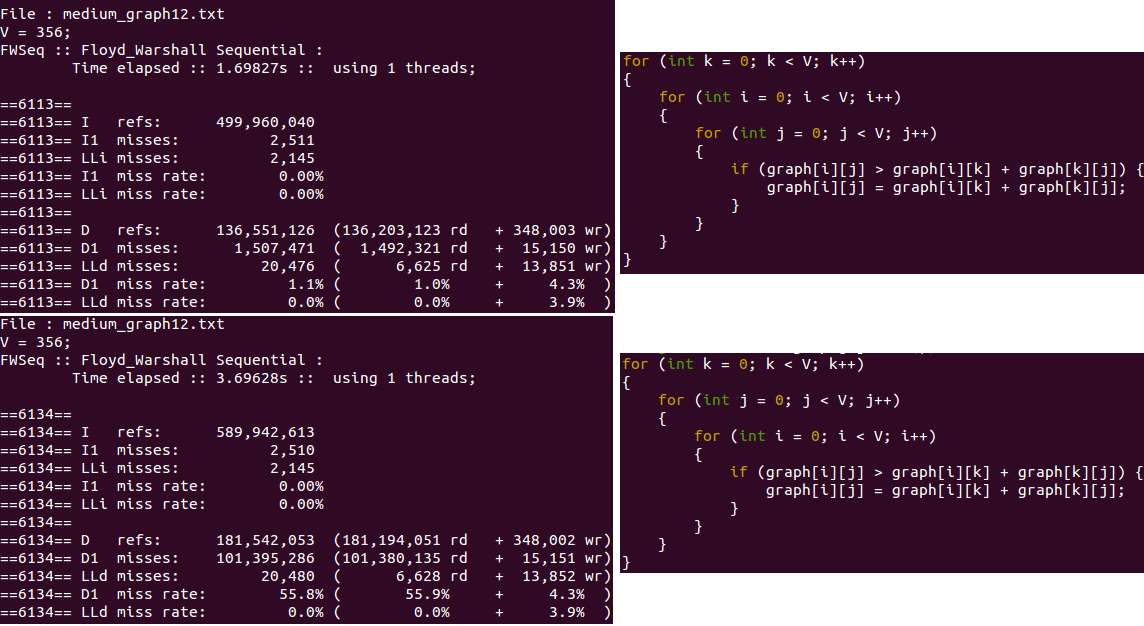
\includegraphics[scale=0.6]{Cache_Importance.png}
\end{center}

Pour expliquer cela, on s'intéresse à la dernière boucle dans chaque cas.\\

Dans le premier cas, graph[i][j] est une constante de la boucle, seulement graph[i][j] et graph[k][j] dépendent de la variable de la boucle. Ainsi, pour charger toutes les valeurs de la boucle, il n'y a qu'à charger les lignes i et k de la matrice.\\

Dans le second cas, graph[i][j] et graph[i][k] dépendent de la variable de la boucle. Mais pour chaque valeur de i, il faut charger en mémoire une nouvelle ligne de la matrice.

\noindent Cela génère beaucoup d'erreurs de cache, et explique pourquoi le second cas est beaucoup plus lent que le premier.

\subsection{L'importance de la représentation spatiale de la mémoire}

Cette partie essaie d'expliquer pourquoi l'algorithme avec la matrice en une dimension est le meilleur.

Comme la taille de la matrice des distances est connue à l'exécution, les tableaux sont dynamiques.

C'est pour cela que j'ai utilisé des vecteurs de vecteurs. Ils fonctionnent comme un tableau 2D en C, avec des pointeurs de pointeurs.

Lorsque que la matrice n'est pas en une dimension, la localisation spatiale en mémoire se perd, car chaque ligne peut être loin de la ligne suivante.

\section{Possibilités d'amélioration}

La première chose à faire est de tester les performances sur une machine plus puissante. Le meilleur algorithme devrait être le FWPTB, avec une taille de bloc égal à la taille du cache. Le script Python \textbf{generate\_blocsize\_analysis.py} peut tester différentes tailles de blocs. Il s'appelle depuis le dossier principal.

D'autre part, il est possible d'implémenter l'algorithme de Floyd-Warshall de manière récursive, avec la représentation en mémoire Z-Morton.

\section{Bibliographie}

Tutoriel OpenMP :

https://computing.llnl.gov/tutorials/openMP/\\

\noindent Algorithme de Floyd-Warshall :

https://www.cs.usfca.edu/galles/visualization/Floyd.html

http://www.mcs.anl.gov/itf/dbpp/text/node35.html

http://www.infor.uva.es/diego/docs/ortega13b.pdf

http://www.cse.buffalo.edu/faculty/miller/Courses/CSE633/Muthuraman-Spring-2014-CSE633.pdf

http://courses.csail.mit.edu/6.884/spring10/projects/kelleyk-neboat-slides.pdf

http://citeseerx.ist.psu.edu/viewdoc/download?doi=10.1.1.40.5378\&rep=rep1\&type=pdf

https://prezi.com/z9eiteeaqxmh/parallel-approach-to-floyd-warshall-algorithm/

https://people.cs.kuleuven.be/george.karachalias/papers/floyd-warshall.pdf

http://moais.imag.fr/membres/marc.tchiboukdjian/pub/thesis.pdf

http://escholarship.org/uc/item/9v89p5wv\#page-10

http://repository.upenn.edu/cgi/viewcontent.cgi?article=1213\&context=hms

https://www.google.com.ar/url?sa=t\&rct=j\&q=\&esrc=s\&source=web\&cd=1\&ved=0ahUKEwjUpeKBxO\_PAhWIH5AKHb2zBLcQFggcMAA\&url=http\%3A\%2F\%2Fwww.cs.technion.ac.il\%2Fitai\%2FCourses\%2FCache\%2FPresentations\%2Foptimizing-gr-algs.ppt\&usg=AFQjCNEidlujtiLvwSzdGqEQ56XNeDyrKA\&cad=rja\\


\noindent Z-Morton order :

https://en.wikipedia.org/wiki/Z-order\_curve\\


\noindent Défauts de cache :

http://valgrind.org/docs/manual/cg-manual.html

http://igoro.com/archive/gallery-of-processor-cache-effects/


\end{document}
